\documentclass[UTF-8]{ctexart}


\usepackage{url}
\usepackage{cite}
\usepackage[version=4]{mhchem}
\usepackage{graphicx}
\usepackage{subfigure}
\usepackage[a4paper,top=2cm,bottom=2cm,right=3cm,left=3cm,marginparwidth=1.75cm]{geometry}
\usepackage{amsmath}

\title{人机交互中的电磁学原理}
\author{闫皓铭 \\ 元培学院 2300017744}
\date{Autumn, 2024}


\begin{document}
\maketitle

\section{引言}
作为整合科学专业的学生,我一直试图在与生物学相关的多学科交叉的领域中,寻找一些和电磁学课程联系紧密的,有趣新颖的话题和对象,作为本次读书报告的主题。
最终决定阅读和“人机交互”相关的书籍,并把我的一些收获总结在这篇报告中。

人机交互在我们的日常生活中已经非常普遍了,这里所谓的“机”,以手机、平板等电子设备为典型代表。
而电子设备中,自然涉及到诸多电磁学知识作为其原理,与此同时,在不同应用场景中,展现出很大的灵活性、多样性与实用性。
而人机交互也离不开人的感官和感觉。交互方式通常涉及“视觉”、“听觉”和“触觉”。
为了实现更好的人机交互效果,相关电子设备的设计都基于人类的生物学特征和基本的生物学原理。

通过相关资料与书目的阅读,我对很多日常中习以为常的设备的工作原理有了更深刻的认识,
对电磁学理论的应用有了更丰富的认识,对生物学相关知识有了更生动的认识。
\section{视觉交互} 
\subsection{显示技术:侧重非主动发光显示机理}
\subsection{触控技术}
\subsubsection{电阻式触控:联系静电场部分知识}
\subsubsection{电容式触控:联系静电场部分知识}
\subsubsection{压电式触控:联系电介质部分知识}
\section{触觉交互}
\subsection{振动的产生机制:联系电磁感应部分知识}
% Figure
 \begin{figure}
    \centering
    \subfigure[fig 1]{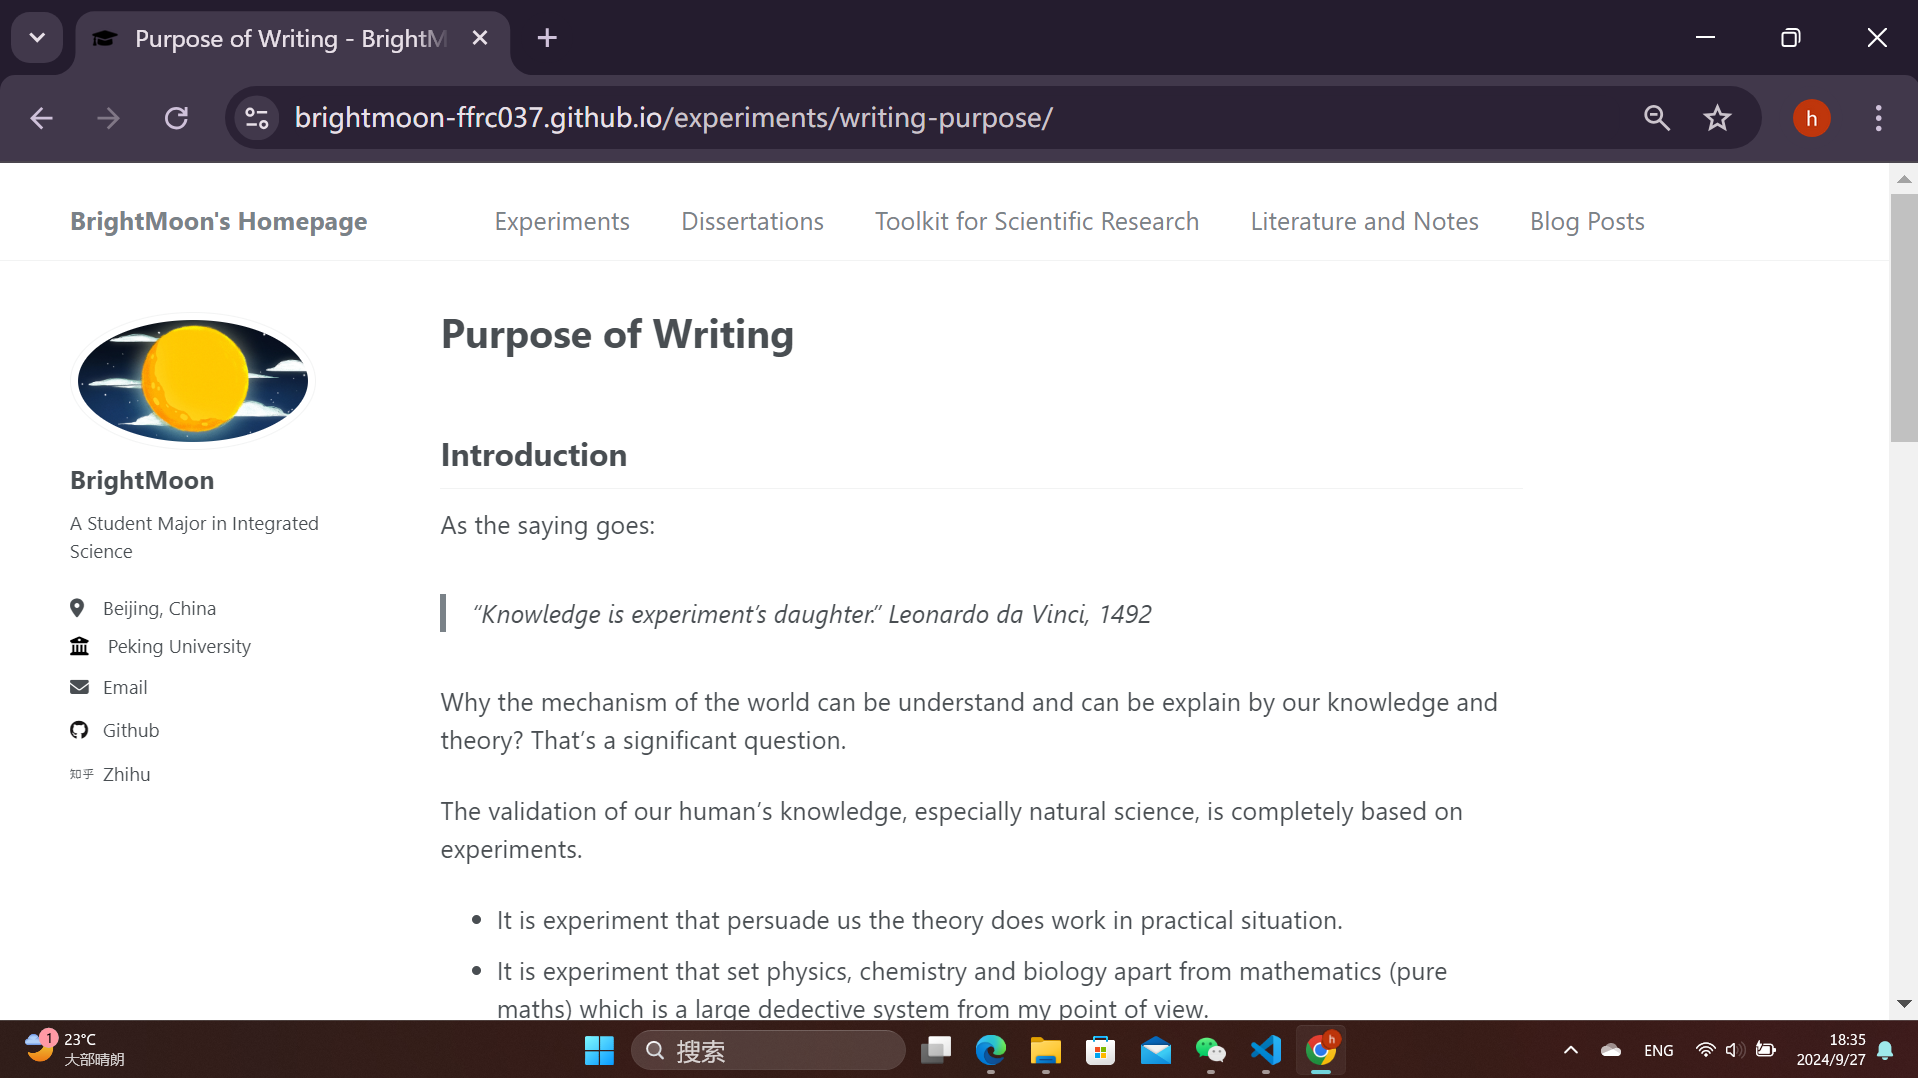
\includegraphics[width=0.7\linewidth]{../Figures/example 1.png}}
    \subfigure[fig 2]{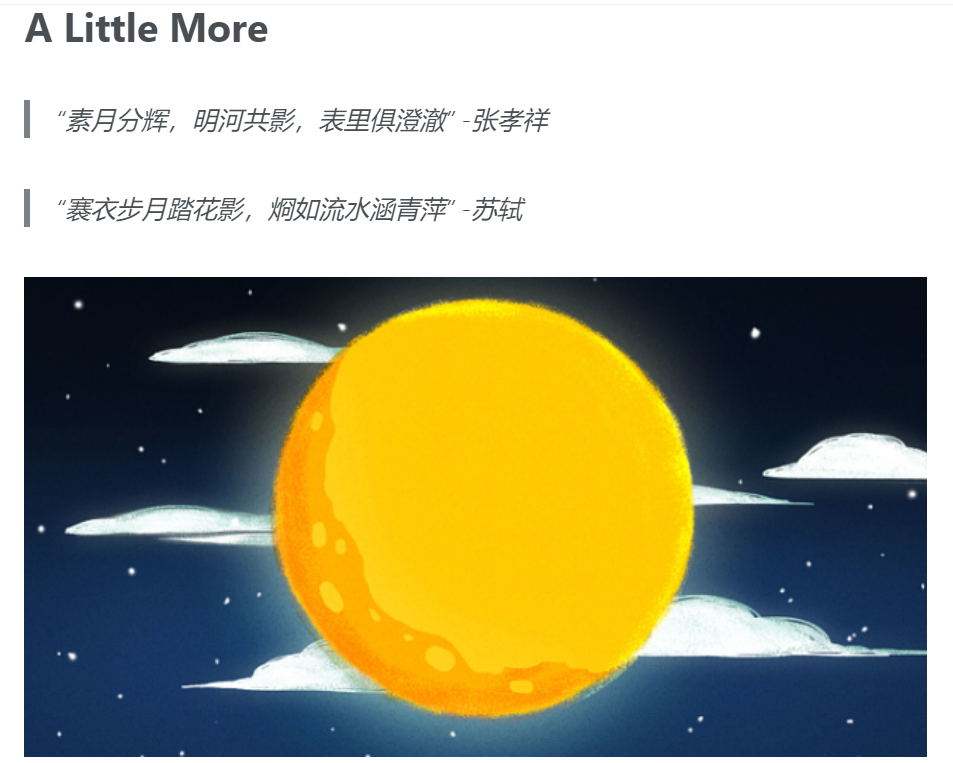
\includegraphics[width=0.7\linewidth]{../Figures/example 2.png}}
    \caption{example 1}  
    \label{example 1}
 \end{figure}

\begin{figure}
    \centering
    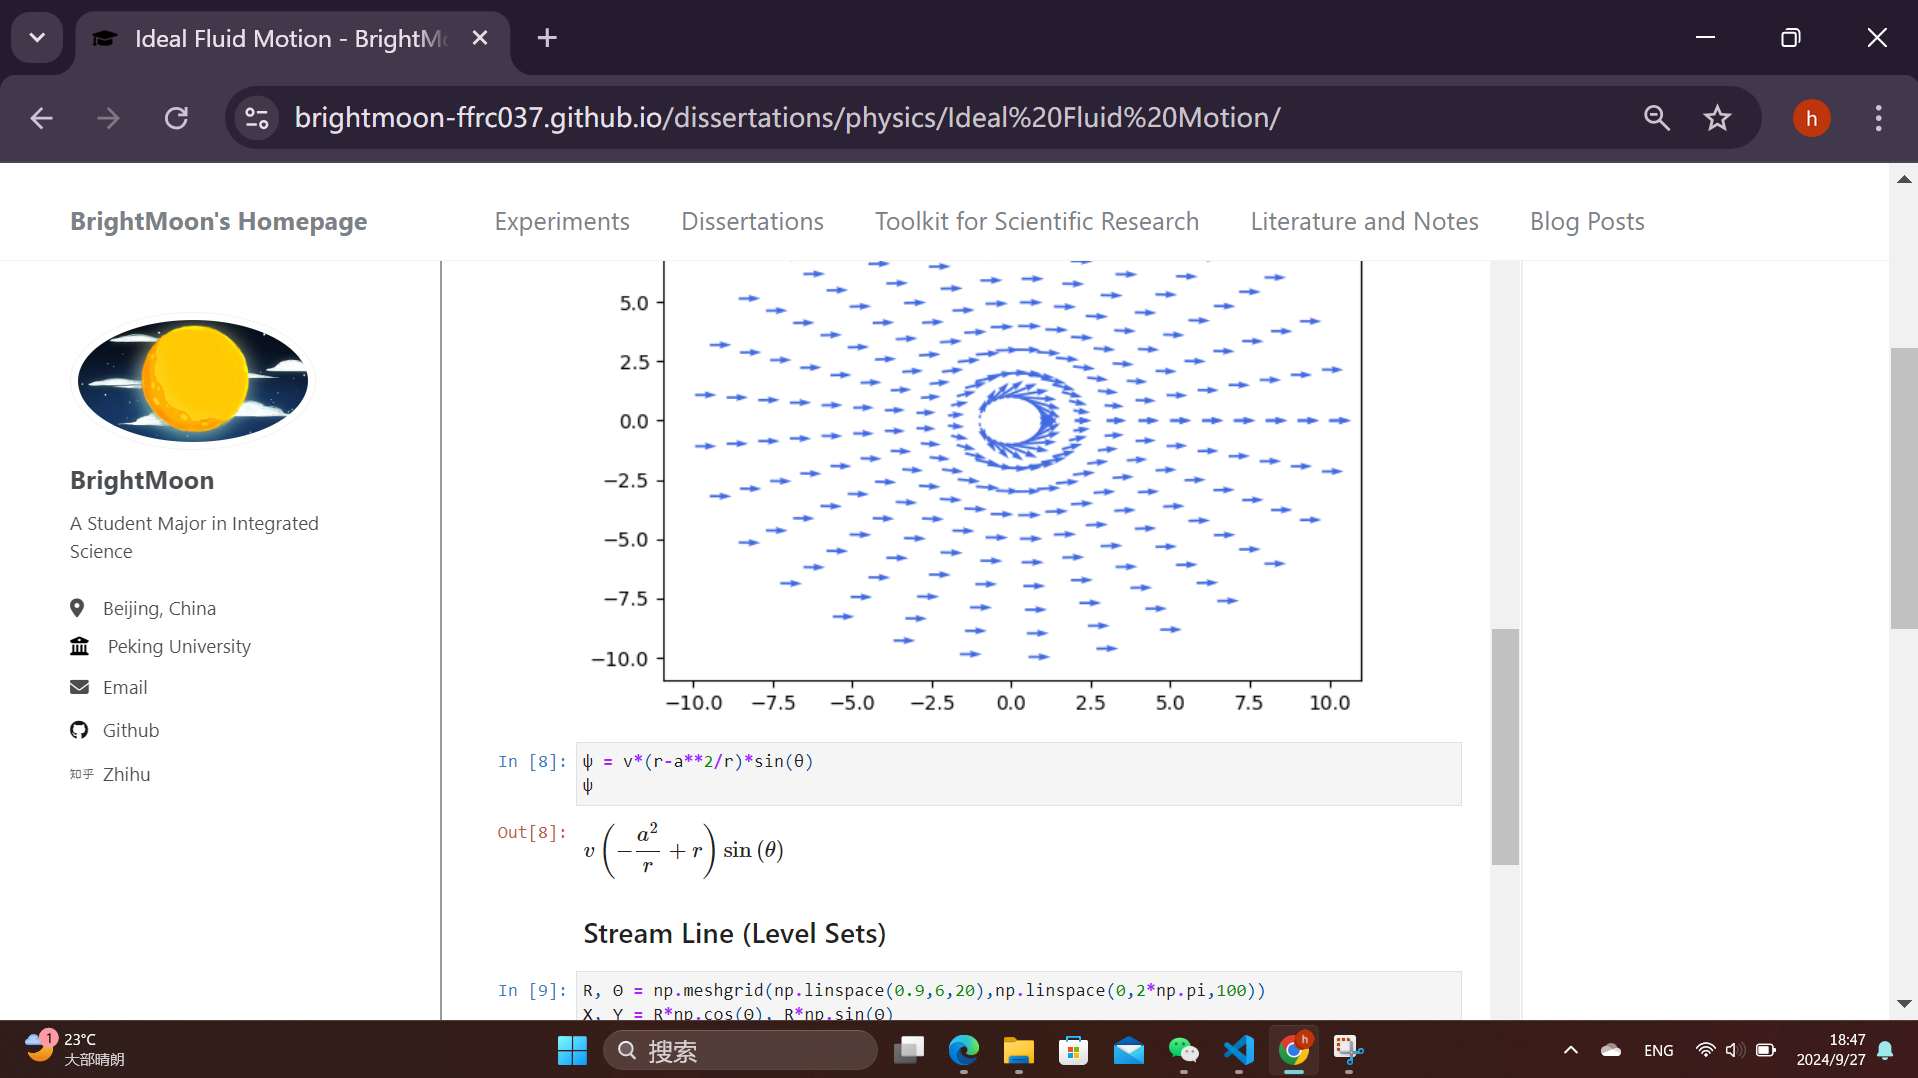
\includegraphics[width=0.7\linewidth]{../Figures/example 3.png}
    \caption{example 2}
    \label{example 2}
\end{figure}

% Table
\begin{table}
    \centering
    \begin{tabular}{|c|c|}\hline
        Column One & Column Two \\ \hline
        Content One & Content One\\ \hline
    \end{tabular}
    \caption{example 3}
    \label{example 3}
\end{table}

% List
\begin{itemize}
    \item item 1
    \item item 2
\end{itemize}


\bibliographystyle{plain}
\bibliography{references}
\end{document}